\subsection{Giao diện công bố khảo sát}

\begin{figure}[H]
    \centering
    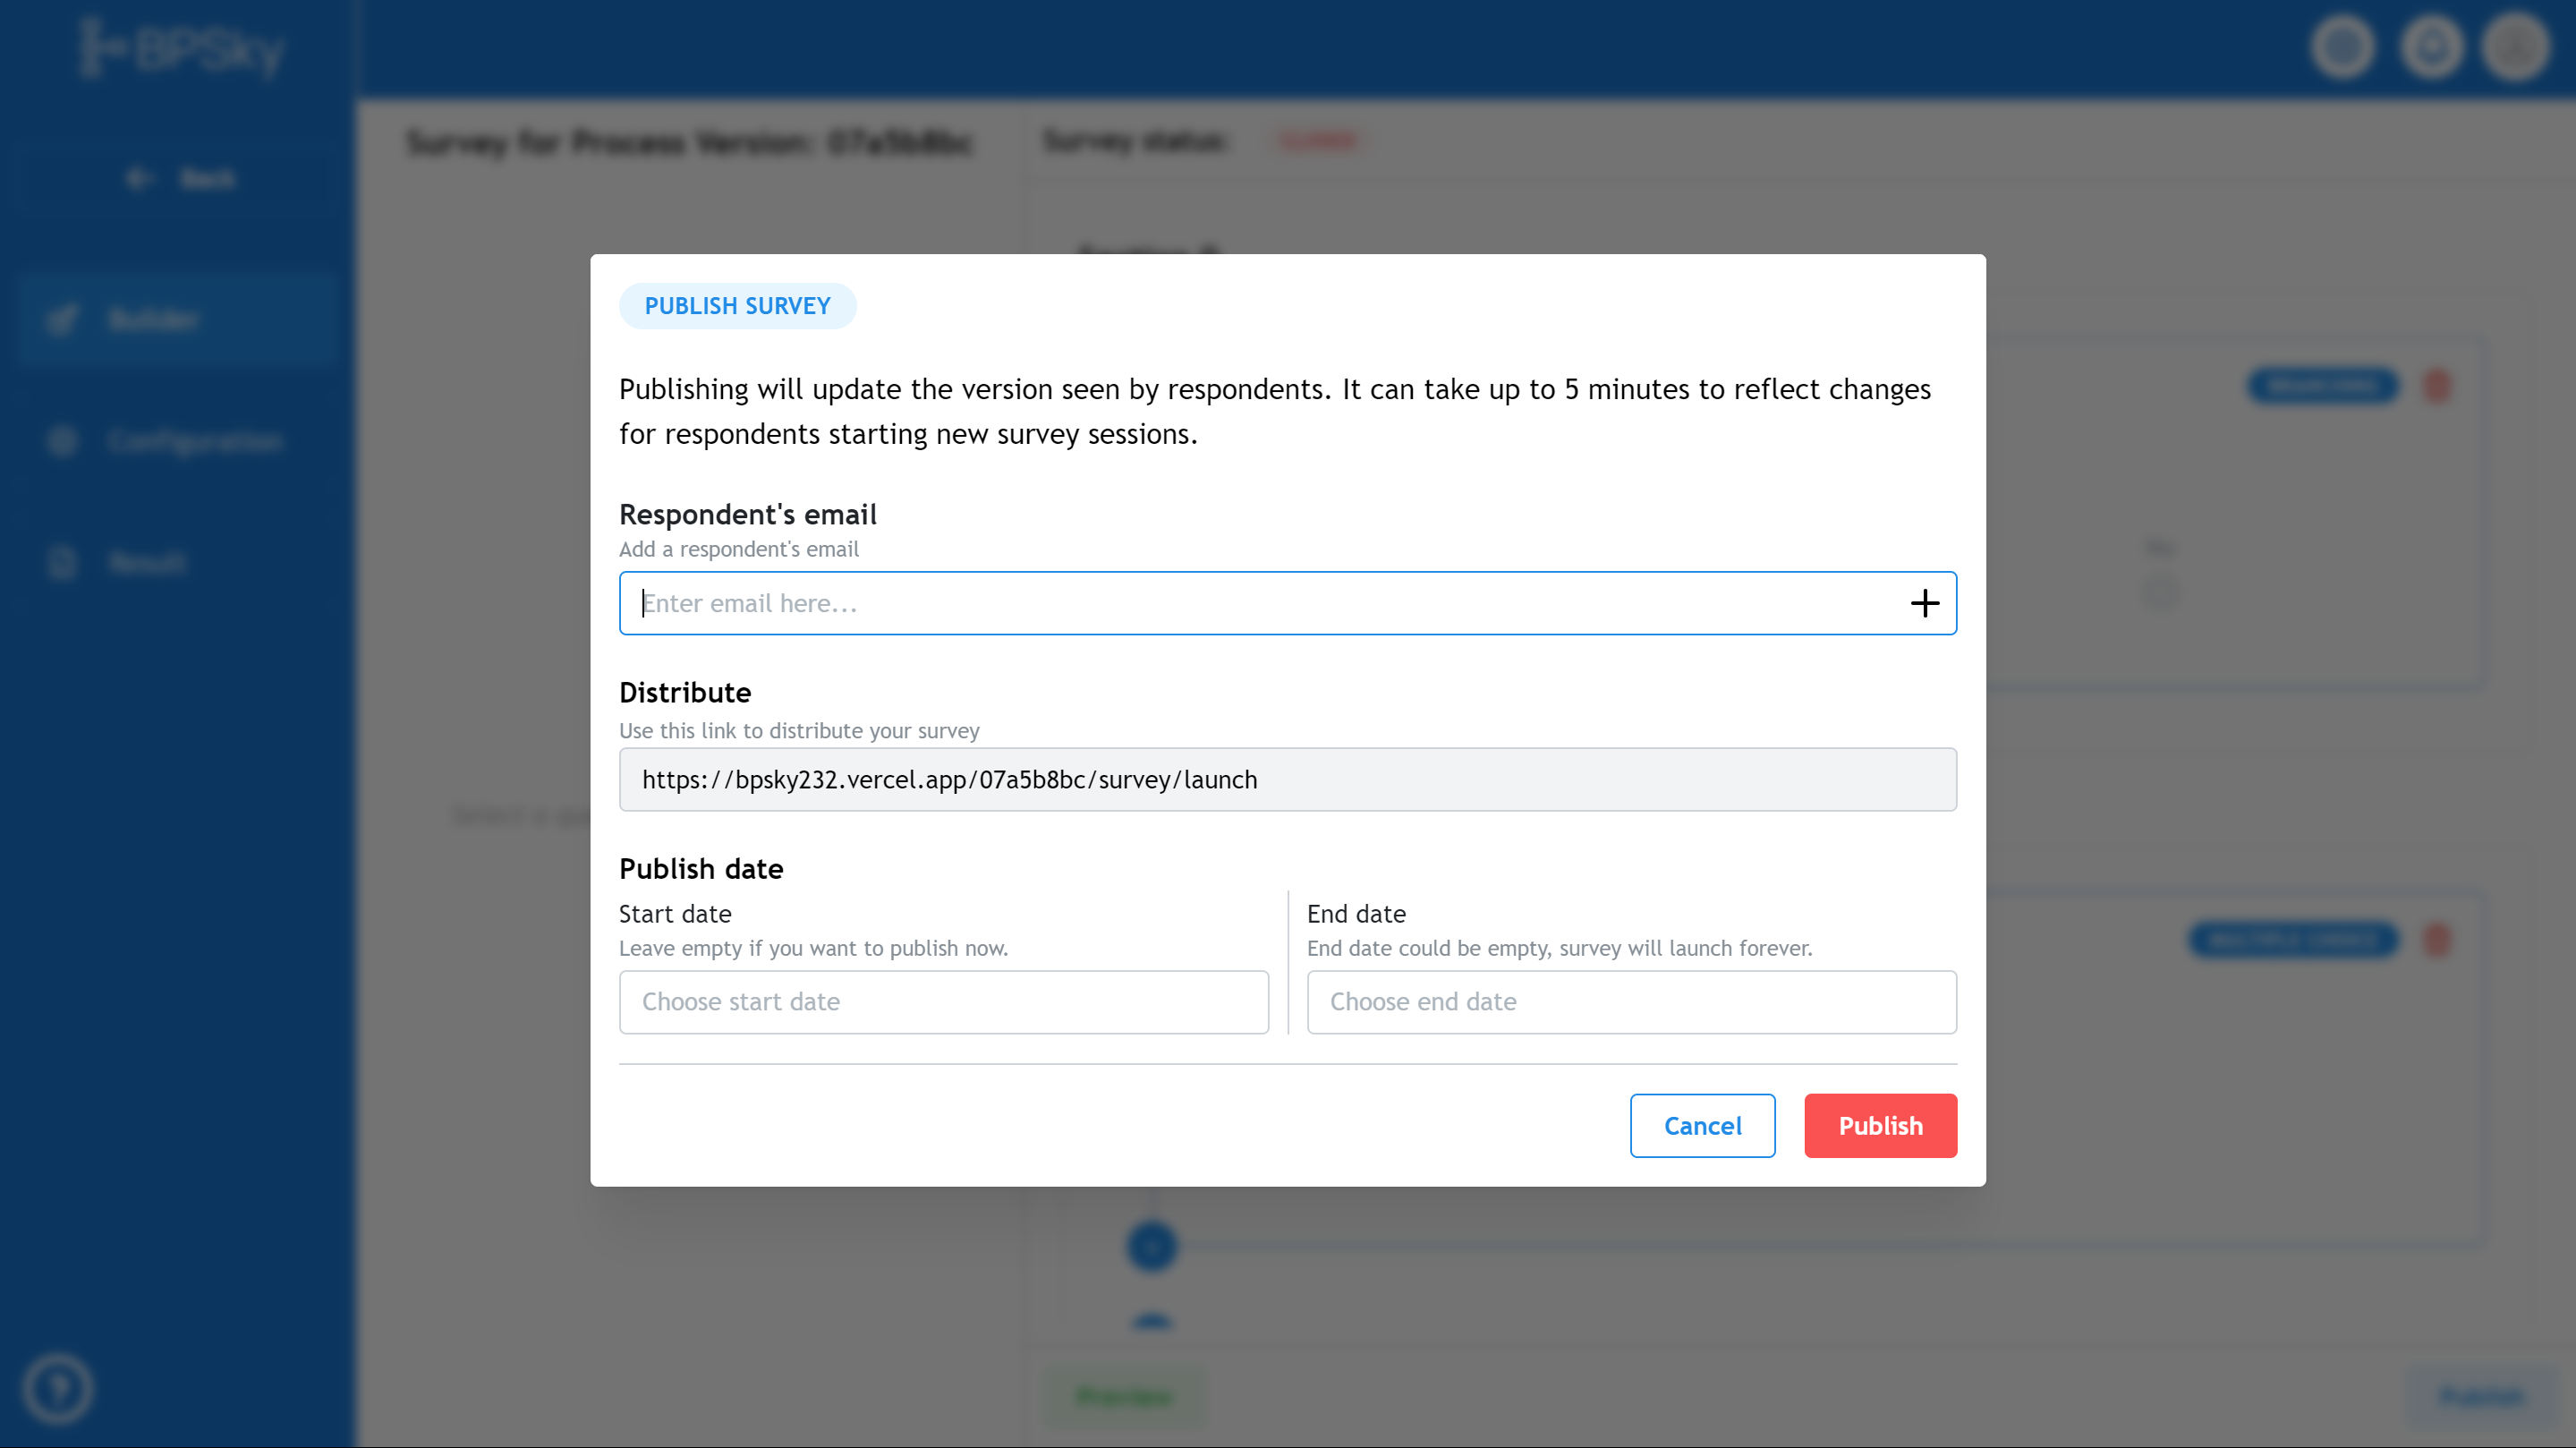
\includegraphics[ width = 0.8\linewidth]{Content/Hiện thực hệ thống/documents/Hiện thực giao diện người dùng/images/SurveyPublish.png}
    \vspace{0.5cm}
    \caption{Giao diện công bố khảo sát}
    \label{fig: Giao diện công bố khảo sát}
\end{figure}

Sau khi người dùng hoàn thành việc cấu hình bảng khảo sát, người dùng có thể chọn mục Publish để công bố bảng khảo sát. Tại đây, người dùng có thể cấu hình các thông tin liên quan tới việc công bố bảng khảo sát như thời gian mở khảo sát, thời gian đóng khảo sát và email của người dùng được gửi thông báo khi khảo sát được mở. Ngoài ra người dùng có thể sử dụng url được tạo sẵn để mời người dùng khác tham gia khảo sát.